\documentclass{beamer}
\usepackage{minted}
\usepackage{hyperref}
\usepackage{graphicx}
\usetheme{Boadilla}
\usecolortheme[]{seahorse}
\hypersetup{
    colorlinks=true,
    linkcolor=black,
    filecolor=magenta,      
    urlcolor=blue,
}
\title{Android Root Detection Evasion}
\author[Roberto Castellotti]{Roberto Castellotti \\ {\small Supervised by: Prof. Giovanni Lagorio}}
\institute{Università di Genova}
\date{2022}
\setbeamertemplate{caption}{\raggedright\insertcaption\par}
\begin{document}

\frame{\titlepage}

\begin{frame}{fundamentals: Android}

    \centering 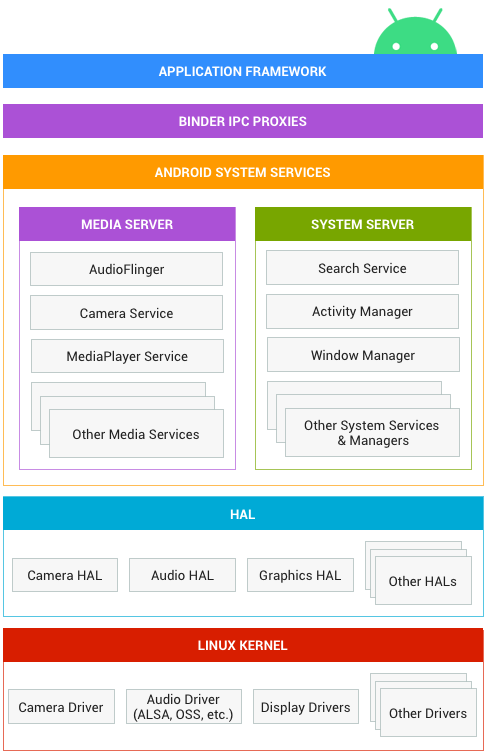
\includegraphics[scale=0.25]{android.png}
    \href{https://source.android.com/devices/architecture}{https://source.android.com/devices/architecture} \\
    by default a user has no root access, despite being the owner of the device
\end{frame}

\begin{frame}{fundamentals: Java to bytecode and back}

    \centering 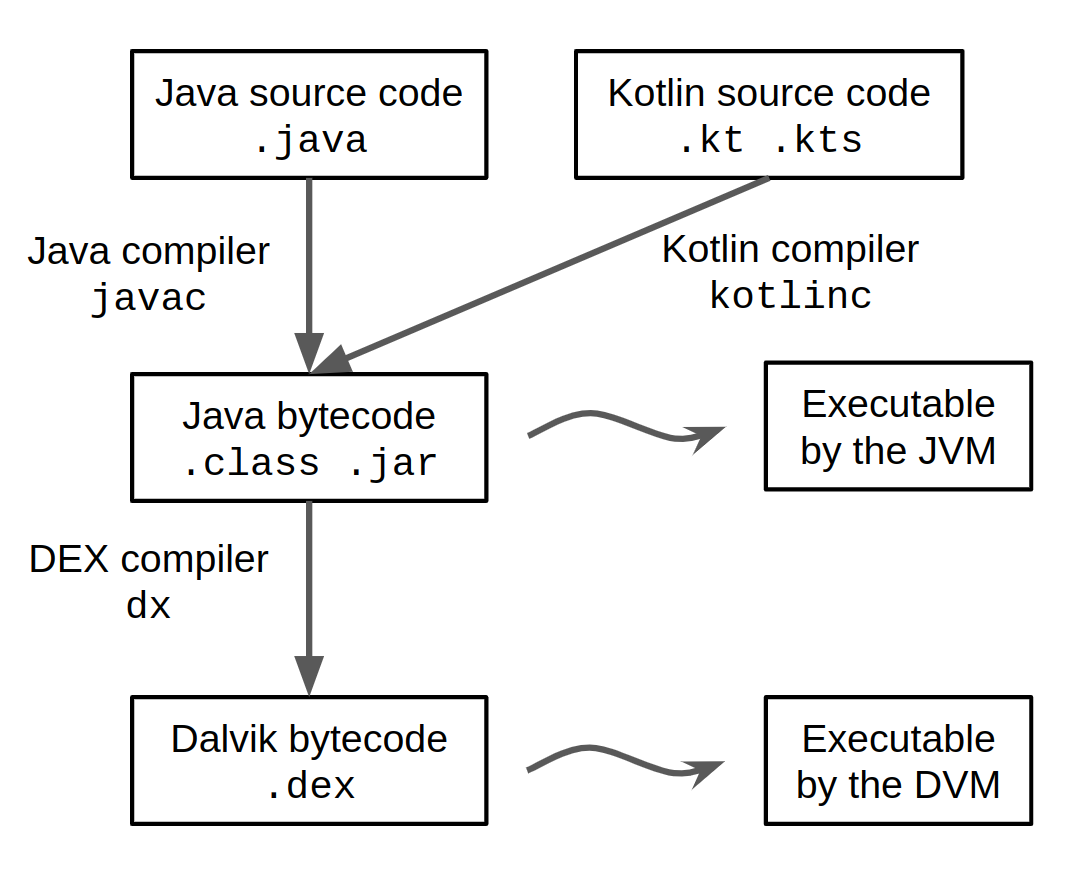
\includegraphics[scale=0.2]{java-to-dex.png}\\
    \href{https://docs.google.com/presentation/d/14nid9QJrSRUd4T_48KZMhWqKT_UdLg7EM-RH0HFQYdM}{MOBISEC 2020 - 10 - Native Code} \\
    at the end of the build process everything is packaged in a \texttt{.apk} file
\end{frame}

% \begin{frame}{\texttt{.dex} and \texttt{.smali}}

%     \begin{itemize}
%         \item up until android 4.4 "KitKat" Dalvik was integral part of software stack
%         \item from android 5.0 "Lollipop" ART is the only included runtime, uses same bytecode and \texttt{.dex} files
%         \item \href{https://github.com/JesusFreke/smali}{JesusFreke/smali}: assembler/disassembler for the dex format used by dalvik, we obtain smali code when decompiling with \texttt{apktool}
%     \end{itemize}

% \end{frame}


% \begin{frame}[fragile]{sample smali code}

% \begin{minted}[fontsize=\scriptsize]{smali}
% .method private static checkRootMethod1()Z
%     .registers 2
%     .line 1
%     sget-object v0, Landroid/os/Build;->TAGS:Ljava/lang/String;
%     if-eqz v0, :cond_e
%     const-string v1, "test-keys"
%     .line 2
%     invoke-virtual {v0, v1}, Ljava/lang/String;->contains(Ljava/lang/CharSequence;)Z
%     move-result v0
%     if-eqz v0, :cond_e
%     const/4 v0, 0x1
%     goto :goto_f
%     :cond_e
%     const/4 v0, 0x0
%     :goto_f
%     return v0
% .end method
% \end{minted}

% \end{frame}


\begin{frame}[fragile]{root detection: how}

    \begin{itemize}[]
        \item check for root management apps (\texttt{com.topjohnwu.magisk})
              \begin{minted}[fontsize=\footnotesize]{java}
import android.content.pm.PackageManager;
import android.content.Context;
private final Context mContext;
PackageManager pm = mContext.getPackageManager();
pm.getPackageInfo(packageName, 0);
\end{minted}
        \item check root cloaking apps {\small (\texttt{com.devadvance.rootcloak},\texttt{de.robv.android.xposed.installer})}
        \item check for dangerous applications (\texttt{com.dimonvideo.luckypatcher})
        \item check for binaries (\texttt{busybox,su})
              \begin{minted}[fontsize=\footnotesize]{java}
File f = new File(path, filename);
boolean fileExists = f.exists();
\end{minted}
        \item check if some paths are writable (\texttt{/system, /sbin, /etc})
              \begin{minted}[fontsize=\footnotesize]{java}
InputStream inputstream = Runtime.getRuntime().exec("mount")
\end{minted}
    \end{itemize}

\end{frame}

\begin{frame}{patch-and-reinstall}

    \begin{enumerate}[]
        \item pull the APK
        \item {\footnotesize \texttt{apktool d app.apk}}
        \item patch
        \item {\footnotesize \texttt{apktool b app}}
        \item sign the APK with {\footnotesize \texttt{apksigner}}
        \item reinstall the patched APK
              % well technically "this" approach needs it in order to pull the apk, but we can still obtain the apk using com.aurora.store
        \item this approach does not require the android device to be rooted
    \end{enumerate}

\end{frame}

\begin{frame}[fragile]{patch-and-reinstall: an example}

    The patching process is usually a matter of finding the methods performing root detection and patching them, here is an example from a popular financial services company's application:
    \begin{figure}
        \centering 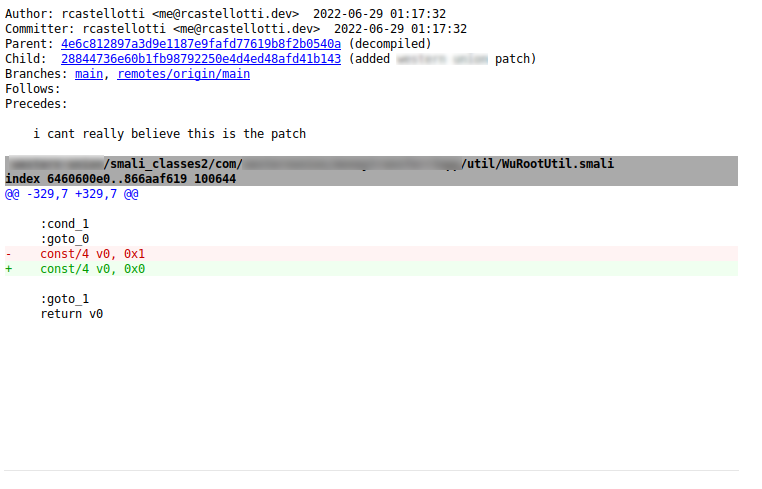
\includegraphics[scale=1.2]{patch.png}
        \caption{patching \mintinline{smali}{.method public static isDeviceRooted()Z} }
    \end{figure}

\end{frame}

\begin{frame}{frida: a dynamic toolkit}

    \begin{itemize}[]
        \item provides ability to inject scripts into black box processes.
        \item portable (Windows, macOS, GNU/Linux, iOS, Android)
        \item \textbf{injected mode}: \texttt{frida-server}: \texttt{frida-core} over TCP
        \item \texttt{frida-core}: a layer that packages up GumJS into a shared library that it injects into existing software, and provides a two-way communication channel for talking to your scripts.
        \item \textbf{on device:} {\footnotesize \texttt{./frida-server-15.1.27-android-arm64}}
        \item \textbf{on computer:} {\footnotesize \texttt{frida -U -l script.js -f com.package.name}}
        \item this approach could be better since it allows to patch applications without losing original package signature
    \end{itemize}

\end{frame}

\begin{frame}[fragile]{frida: \texttt{script.js}}
    \begin{minted}[fontsize=\tiny]{javascript}
Java.perform(function () {
  var PackageManager = Java.use("android.app.ApplicationPackageManager");
  var NativeFile = Java.use("java.io.File");
  var Runtime = Java.use("java.lang.Runtime");

  PackageManager.getPackageInfo.overload(
    "java.lang.String",
    "int"
  ).implementation = function (pname, flags) {
      send("Bypass root check for package: " + pname);
      pname = "set.package.name.to.a.fake.one.so.we.can.bypass.it";
    }
    return this.getPackageInfo
      .overload("java.lang.String", "int")
      .call(this, pname, flags);
  };

  NativeFile.exists.implementation = function () {
    var name = NativeFile.getName.call(this);
      send("Bypass return value for binary: " + name);
      return false;
  };
});

\end{minted}

    \centering{partially adapted from \href{https://codeshare.frida.re/@dzonerzy/fridantiroot/}{@dzonerzy/fridantiroot}}

\end{frame}

\begin{frame}[fragile]{com.revolut.revolut (fintech)}

    \begin{columns}
        \column{0.5\textwidth}
        \begin{figure}
            \centering
            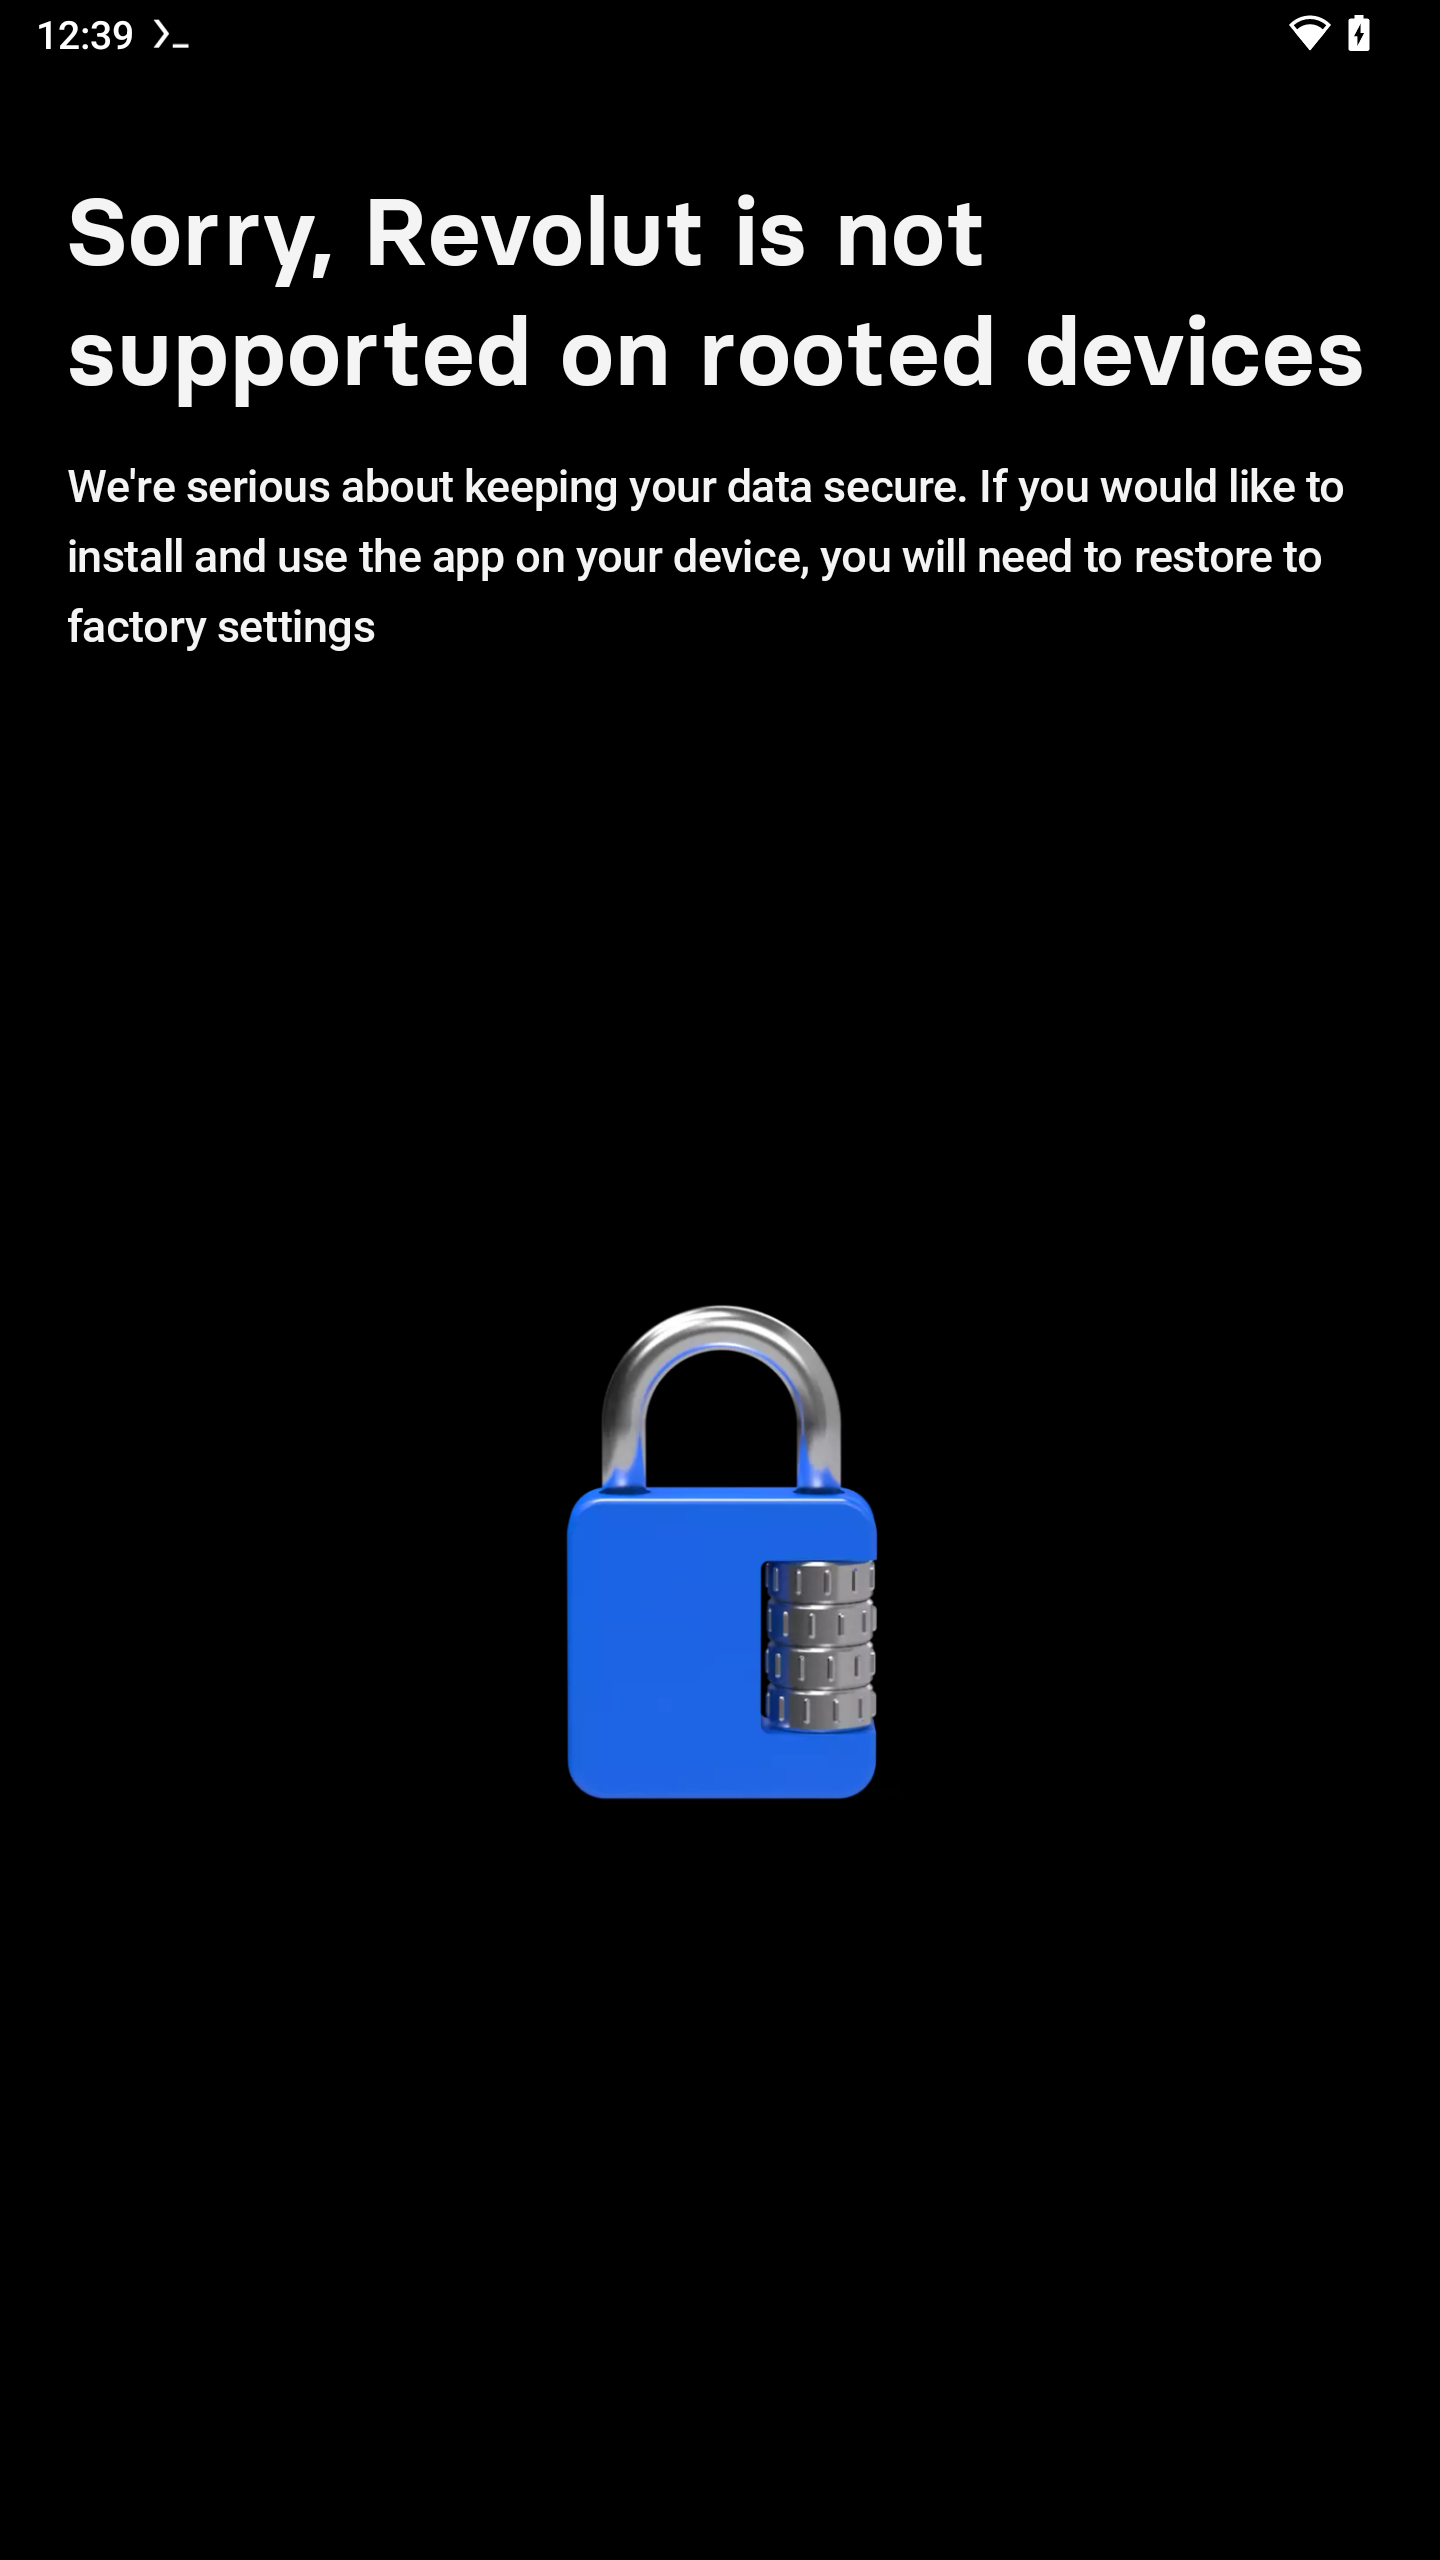
\includegraphics[scale=0.07]{revolut.png}
            \caption{original APK}
        \end{figure}
        \column{0.5\textwidth}
        \begin{figure}
            \centering
            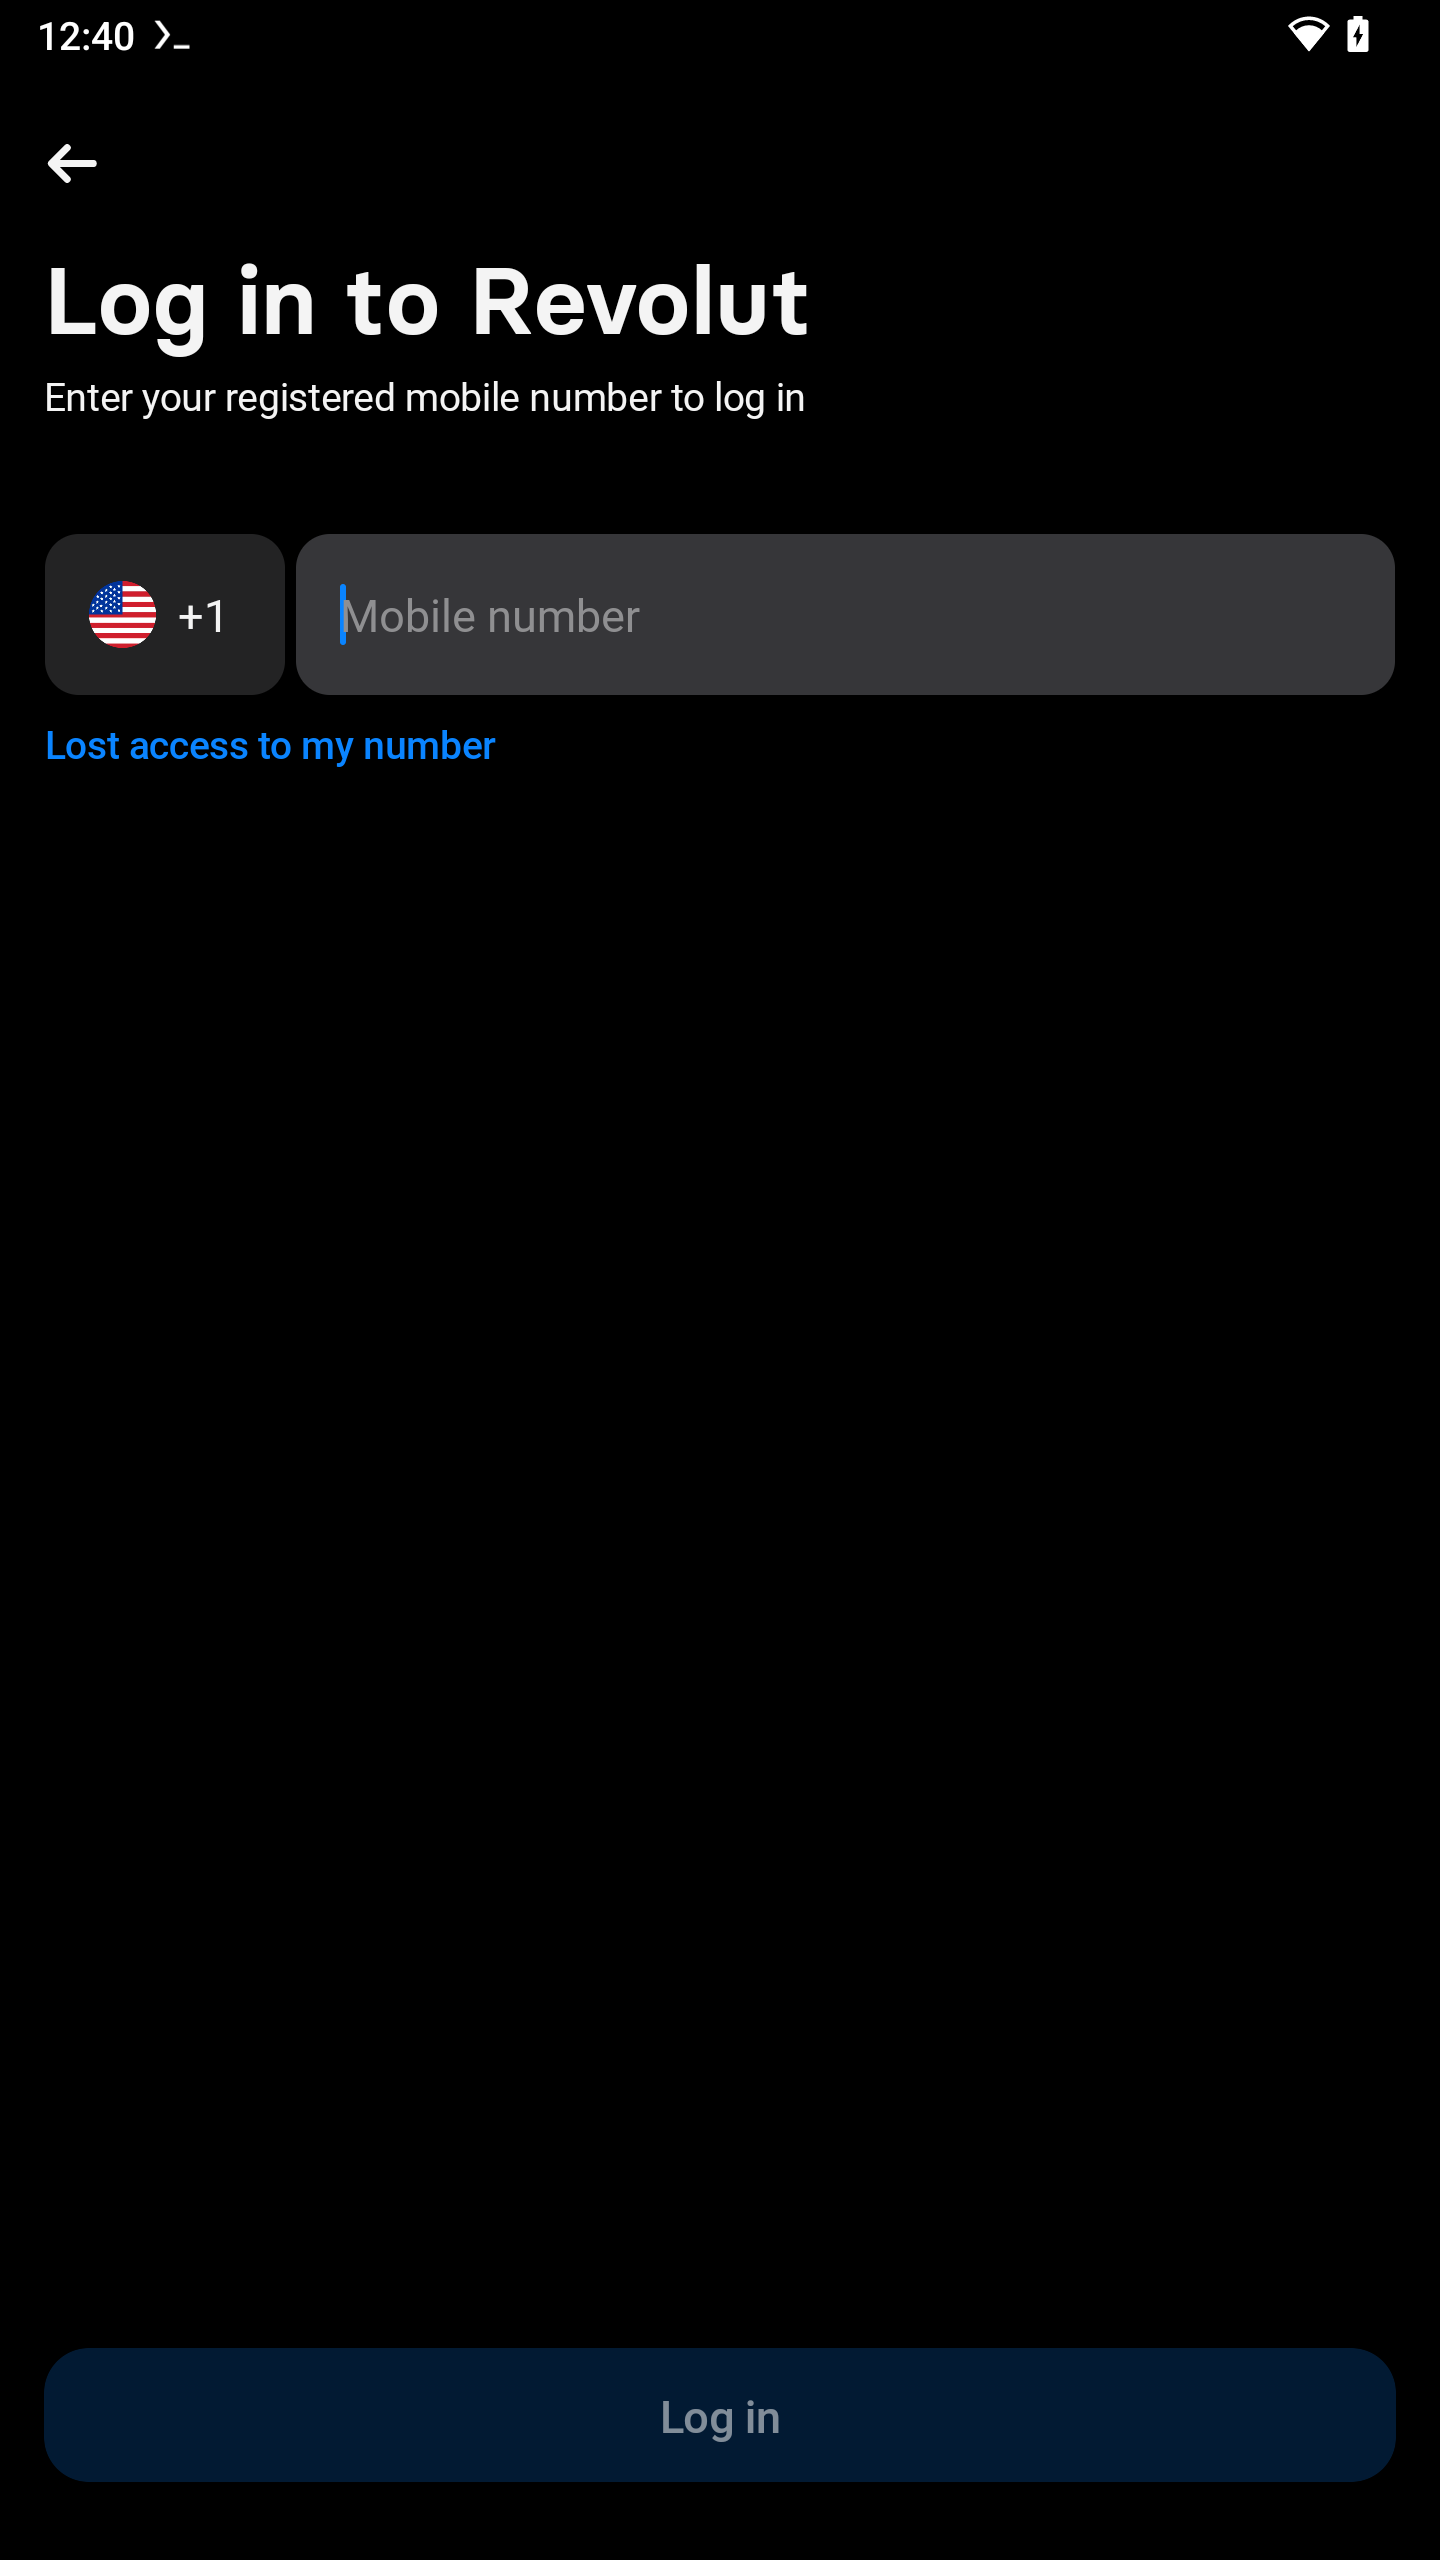
\includegraphics[scale=0.07]{revolut-patched.png}
            \caption{patched}
        \end{figure}
    \end{columns}
\end{frame}

\begin{frame}[fragile]{com.scottyab.rootbeer.sample}

    \begin{columns}
        \column{0.5\textwidth}
        \begin{figure}
            \centering
            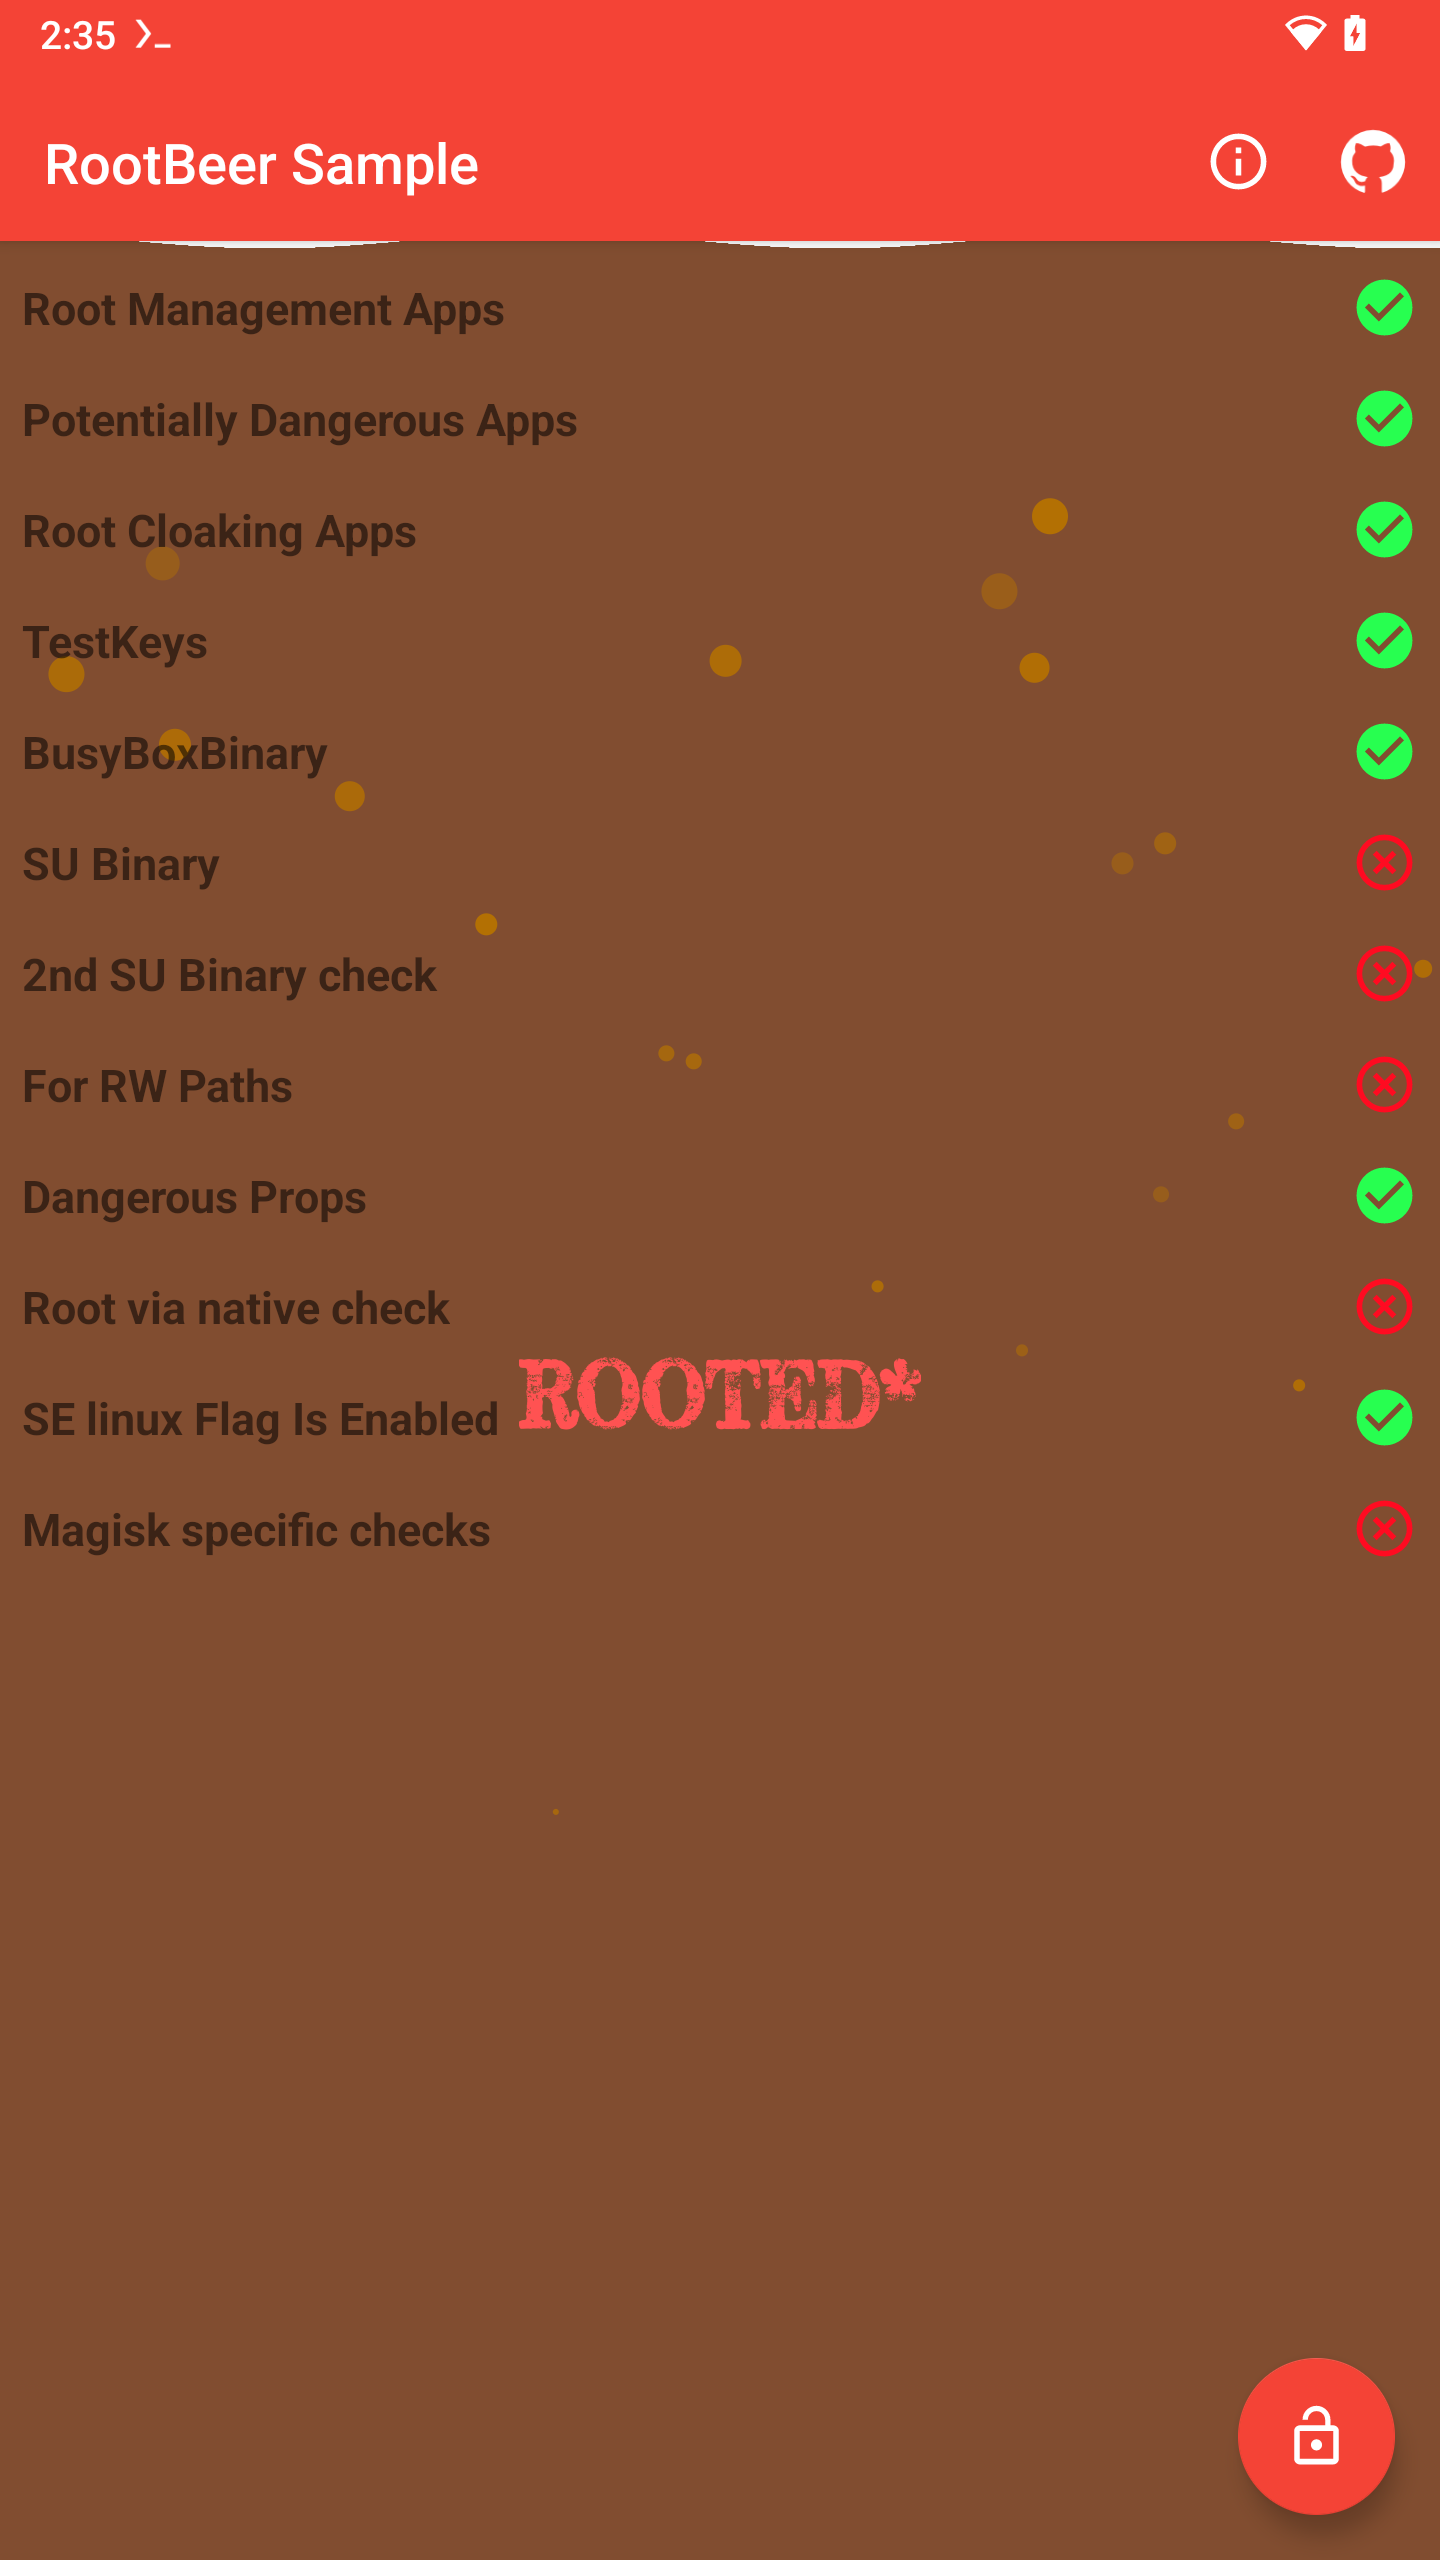
\includegraphics[scale=0.07]{rootbeer.png}
            \caption{original APK}
        \end{figure}
        \column{0.5\textwidth}
        \begin{figure}
            \centering
            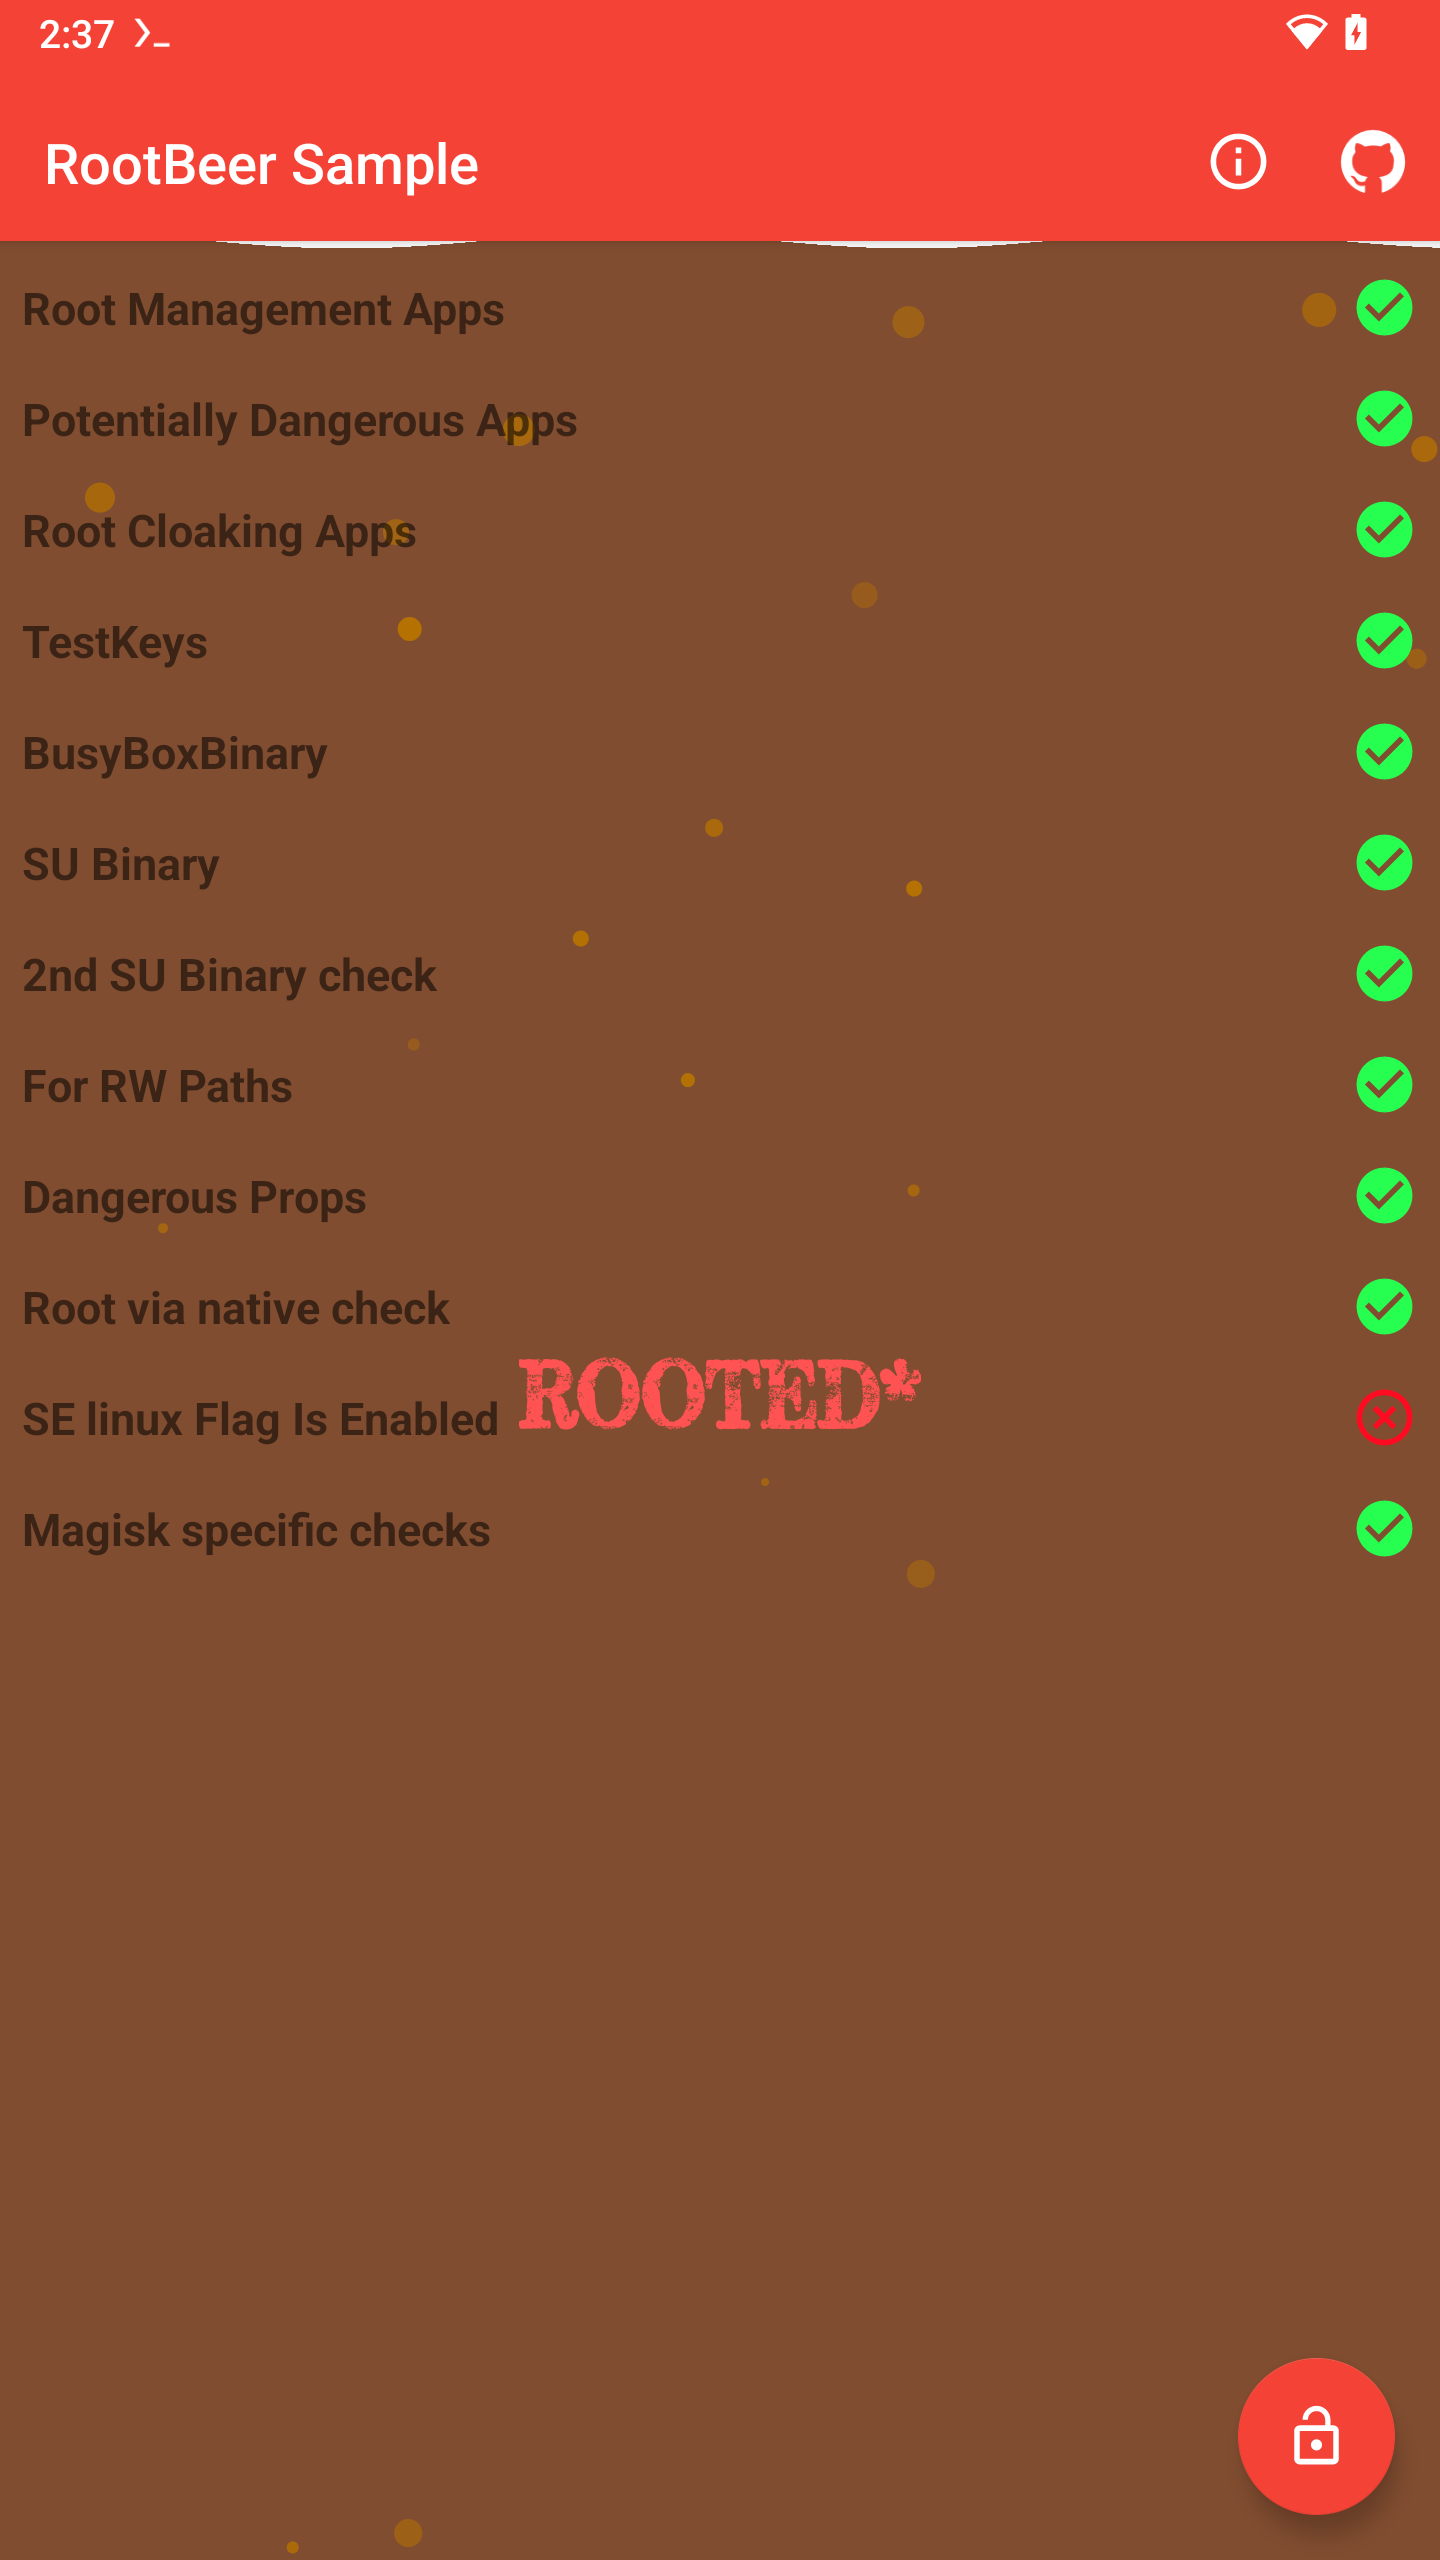
\includegraphics[scale=0.07]{rootbeer-patched.png}
            \caption{patched}
        \end{figure}
    \end{columns}
\end{frame}

\begin{frame}[fragile]{a popular financial services company's application}

    \begin{columns}
        \column{0.5\textwidth}
        \begin{figure}
            \centering
            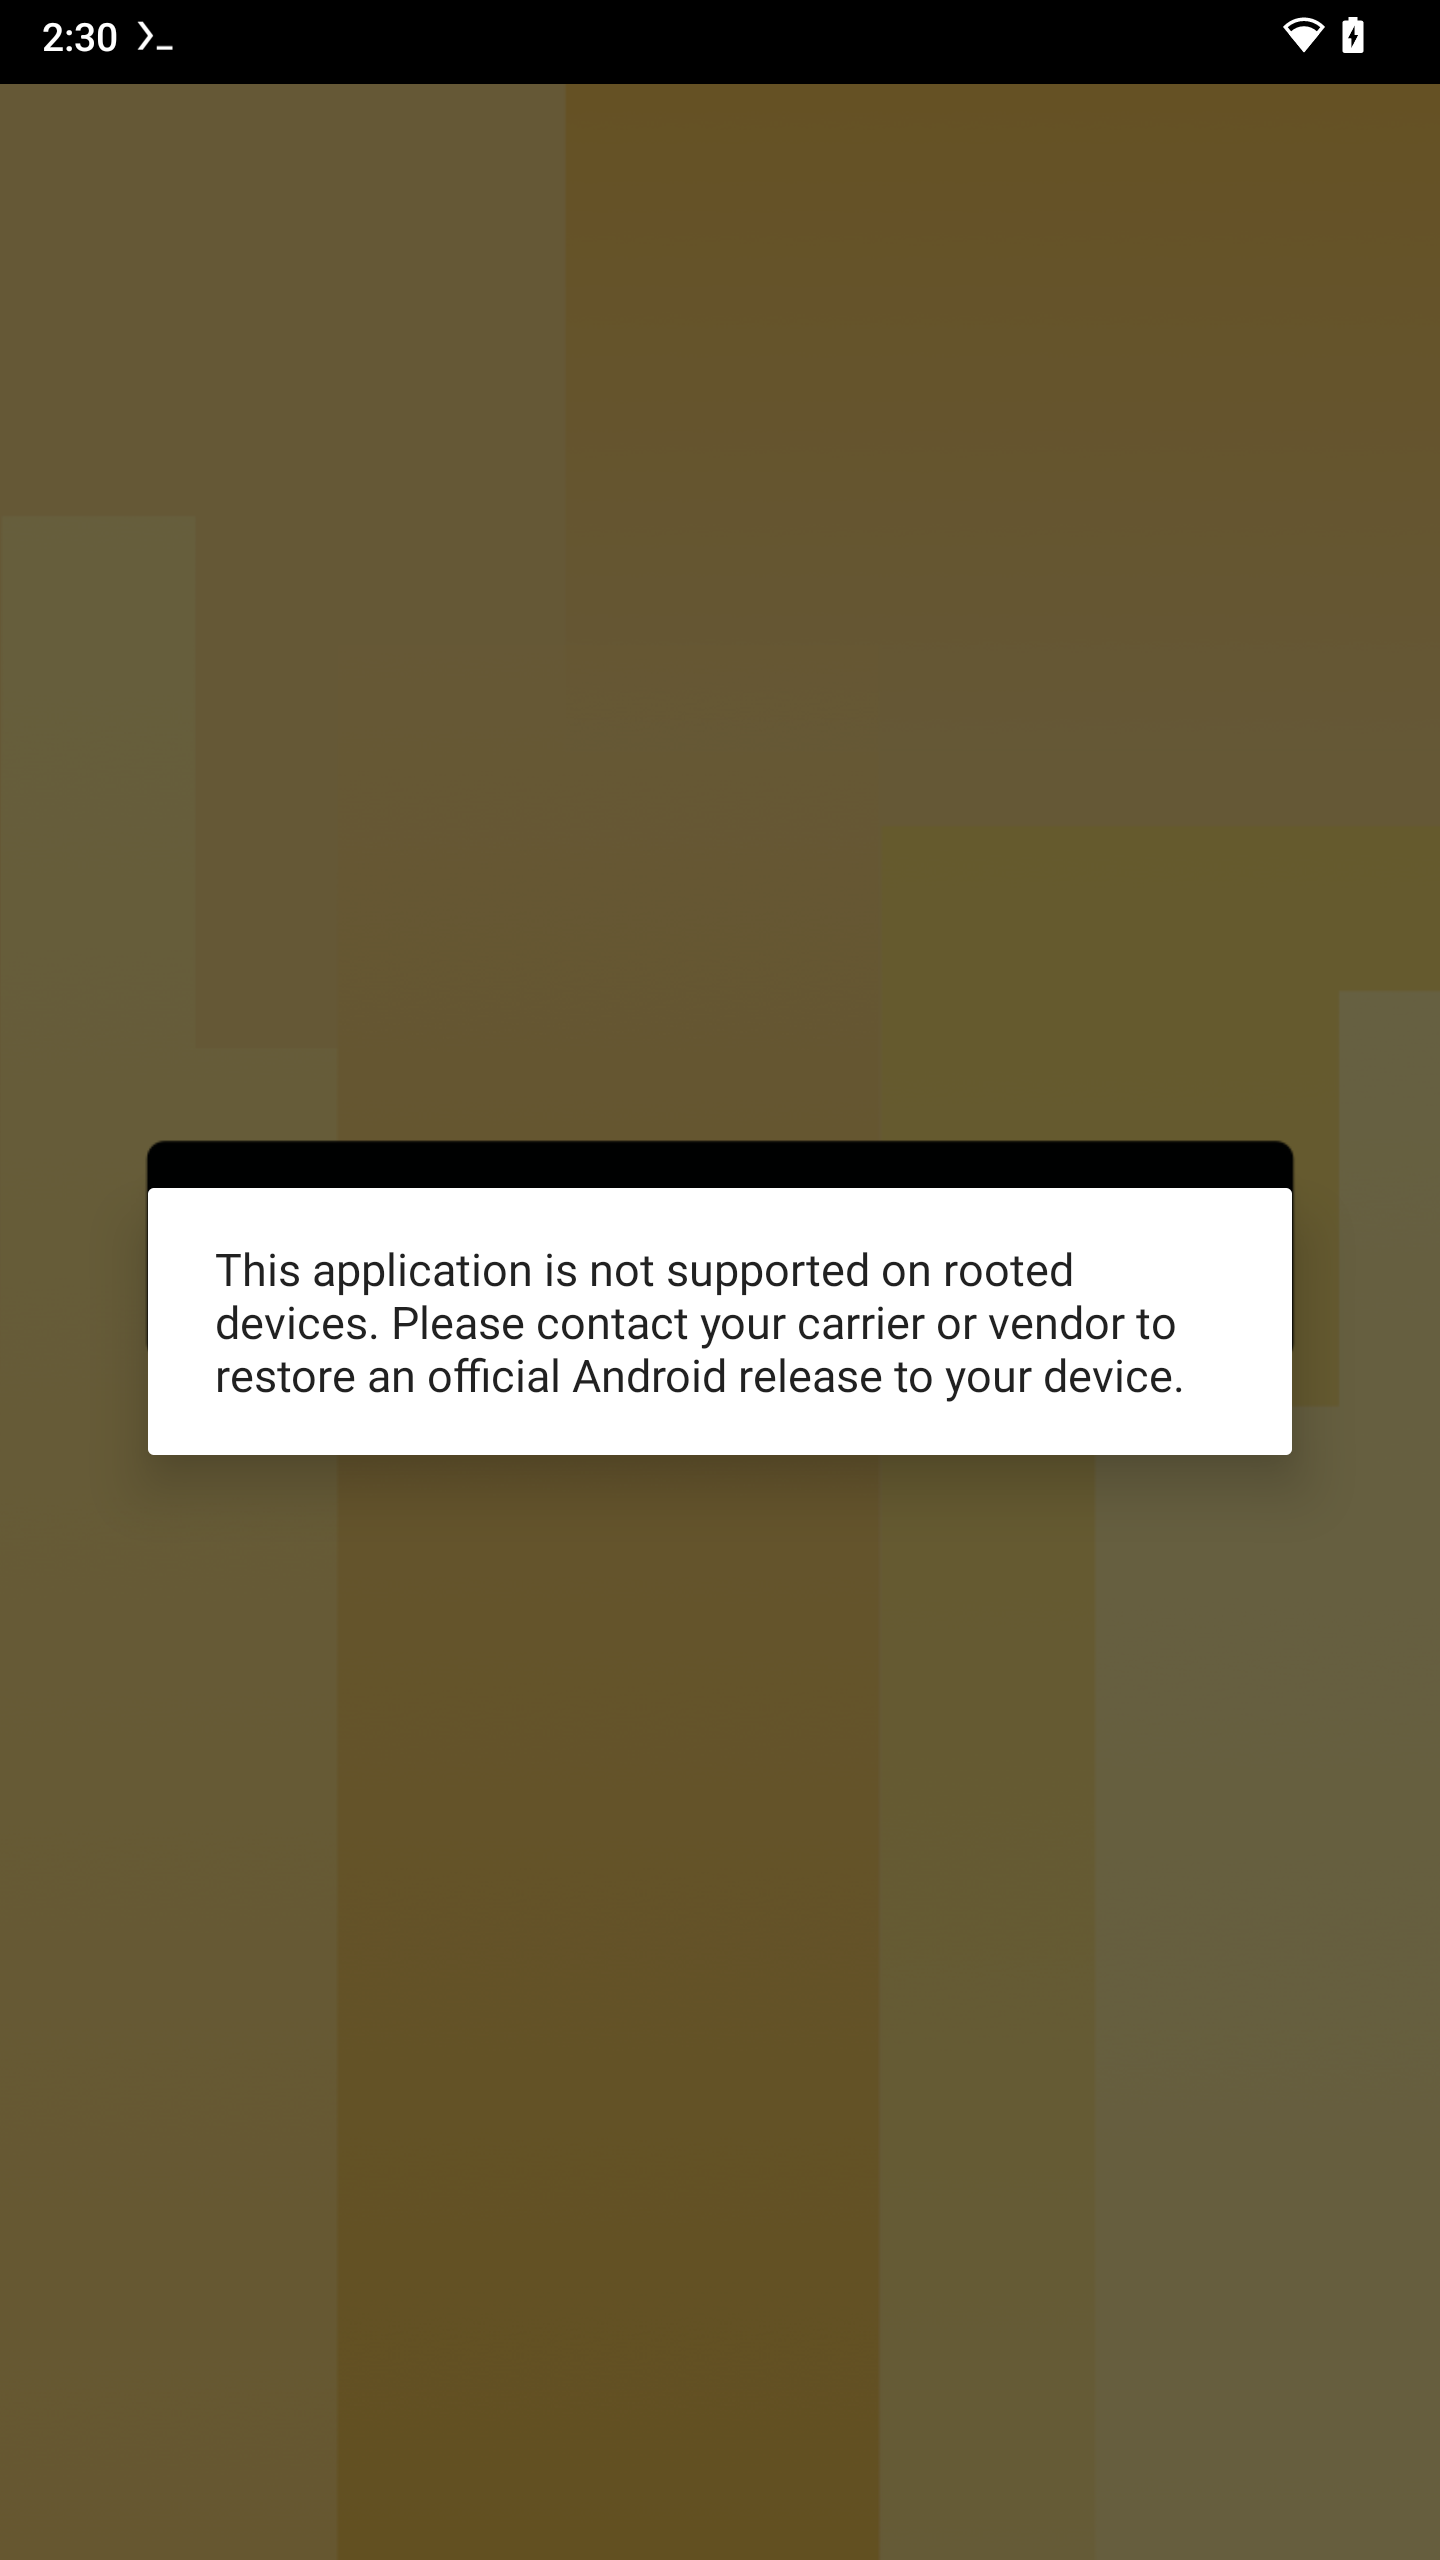
\includegraphics[scale=0.07]{wu.png}
            \caption{original APK}
        \end{figure}
        \column{0.5\textwidth}
        \begin{figure}
            \centering
            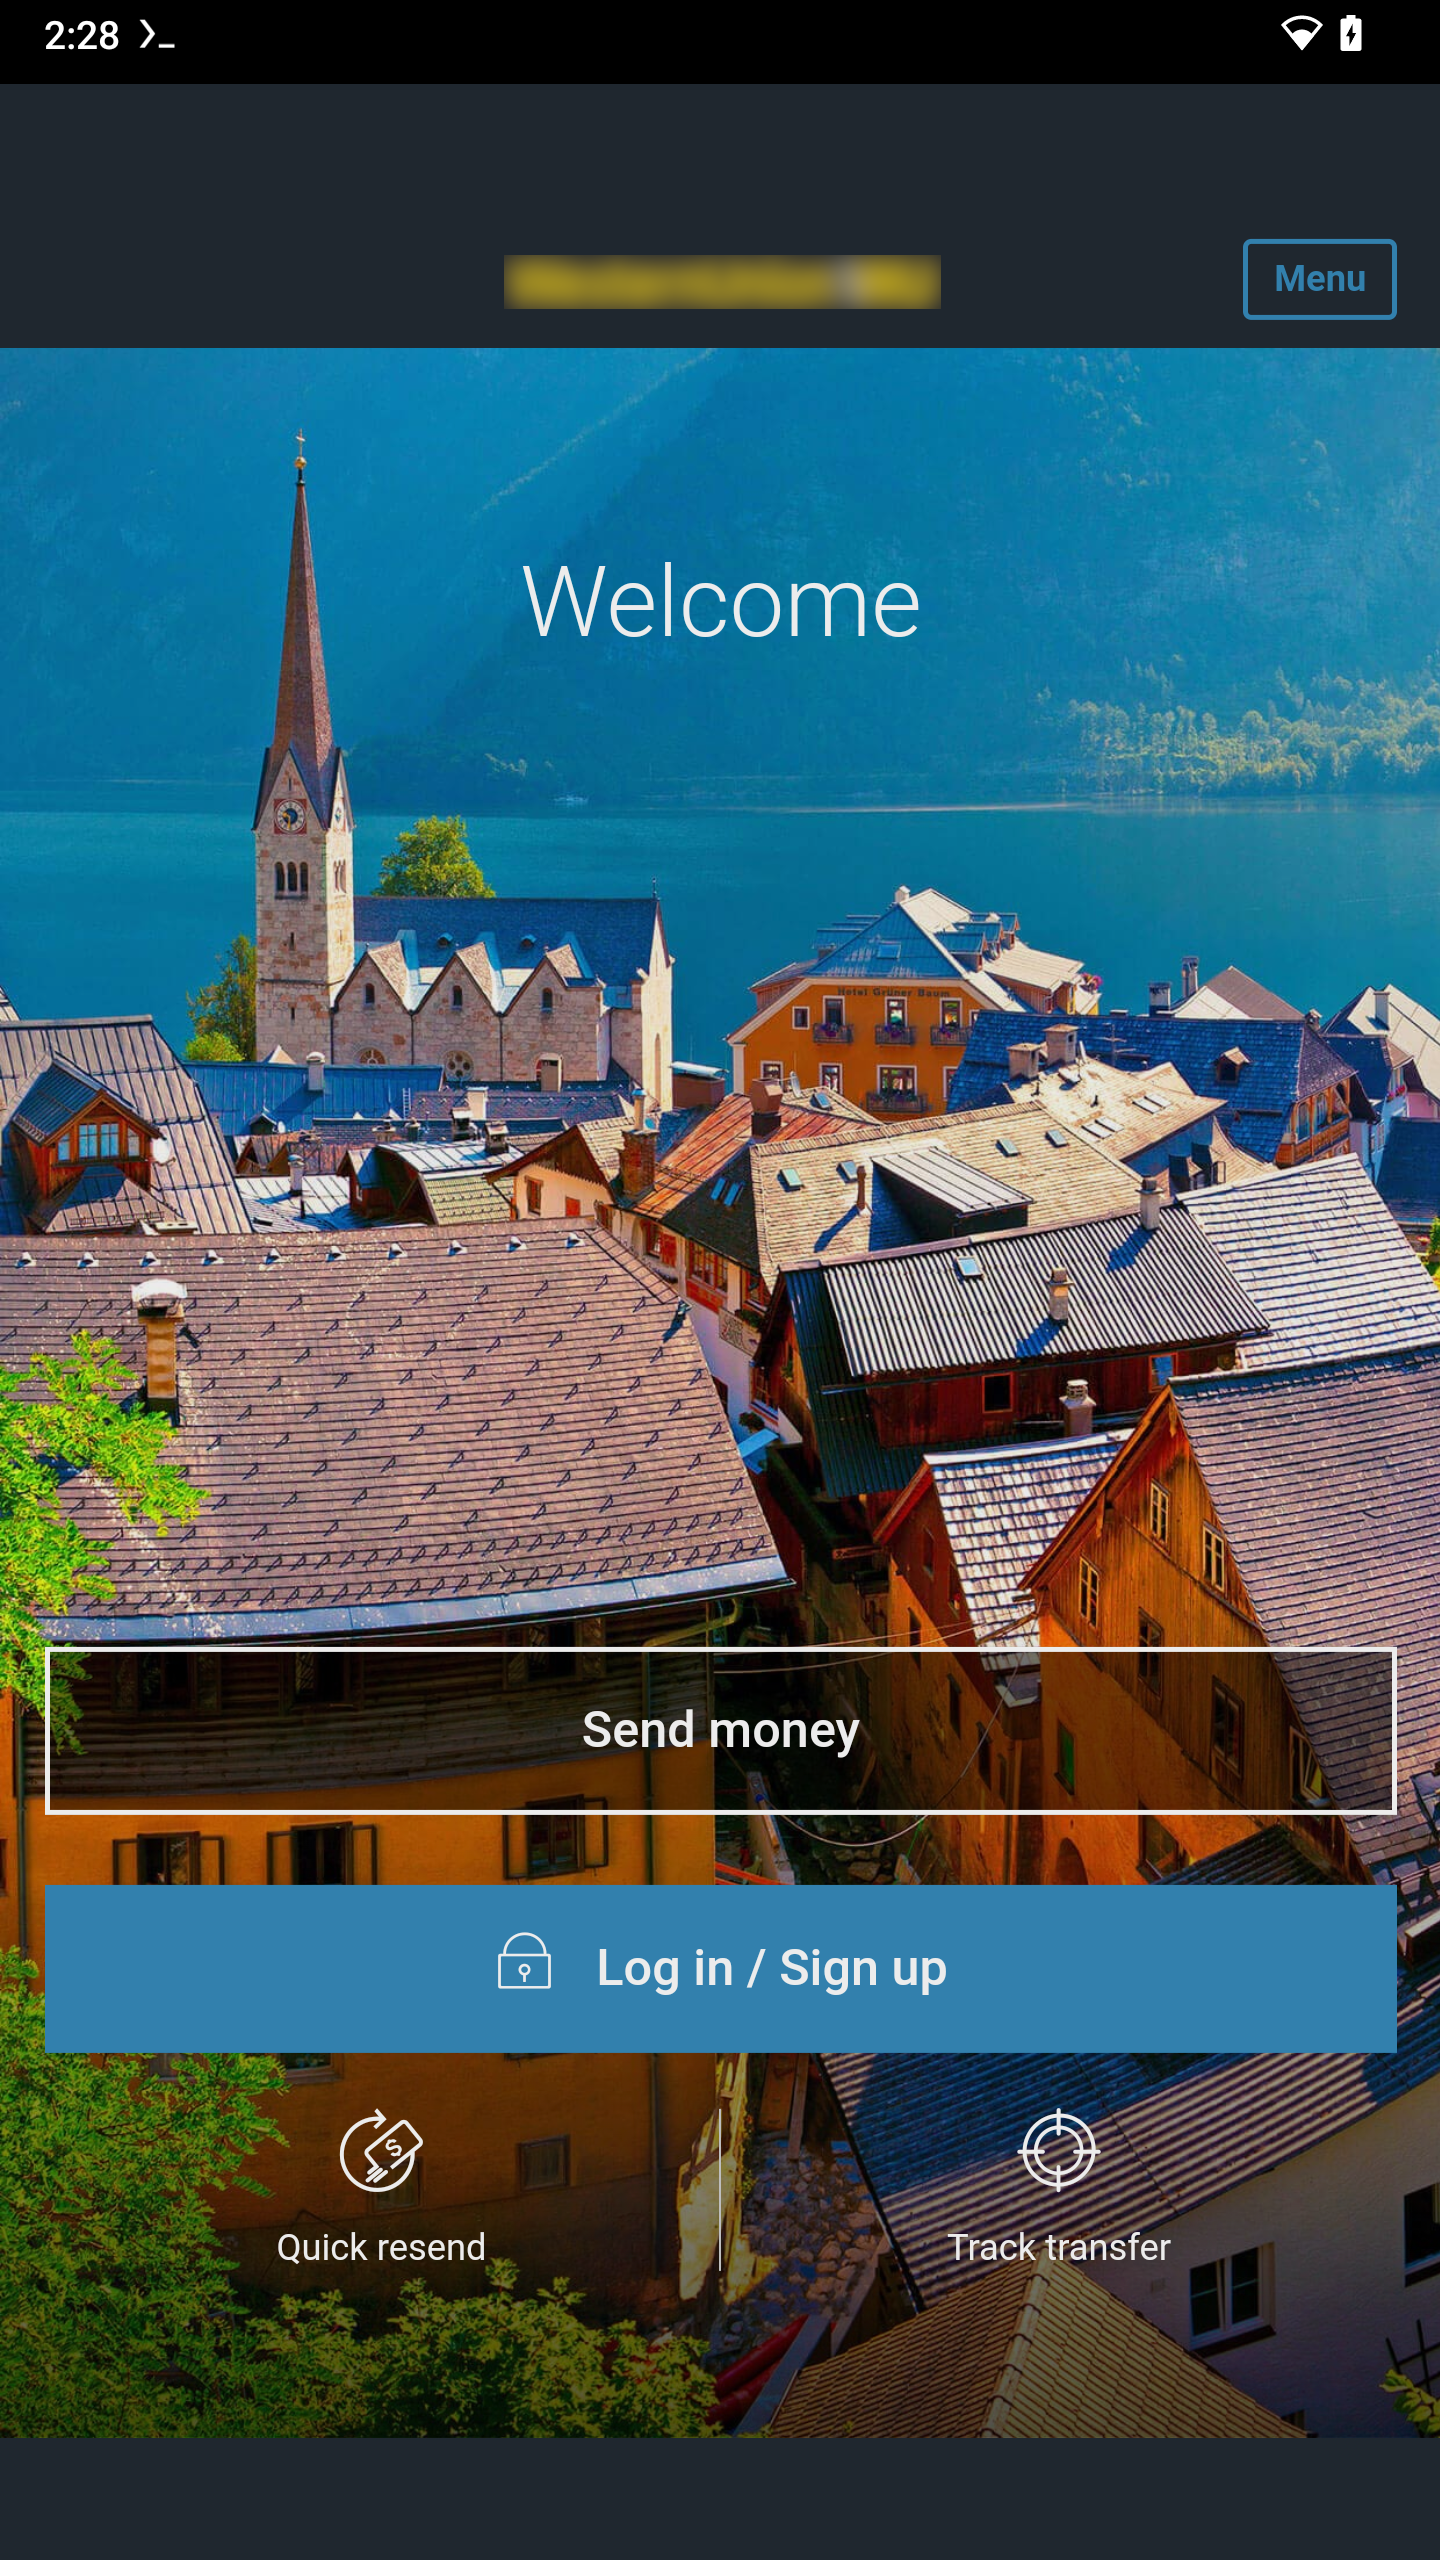
\includegraphics[scale=0.07]{wu-patched.png}
            \caption{patched}
        \end{figure}
    \end{columns}
\end{frame}

\begin{frame}{}
    \centering \Huge
    \emph{Thank You for your attention, Questions?}
\end{frame}

\begin{frame}{tools and sources}

    \begin{itemize}
        \item \href{https://developer.android.com/studio}{Android Studio}
        \item \href{https://github.com/iBotPeaches/Apktool}{iBotPeaches/Apktool}:
              A tool for reverse engineering Android apk files
        \item \href{https://github.com/skylot/jadx}{skylot/jadx}: Dex to Java decompiler
        \item \href{https://github.com/scottyab/rootbeer}{scottyab/rootbeer}: root checking Android library and sample app
        \item \href{https://en.wikipedia.org/wiki/Dalvik}{https://en.wikipedia.org/wiki/Dalvik}
        \item \href{https://source.android.com/devices/tech/dalvik/dalvik-bytecode.html}{Dalvik Bytecode}
        \item \href{https://source.android.com/devices/architecture/modular-system/art}{Anroid Runtime}
        \item \href{https://developer.android.com/guide/components/fundamentals}{https://developer.android.com/guide/components/fundamentals}
    \end{itemize}

\end{frame}

\end{document}